\clearpage
\twocolumn[{%
\subsection{Item selection from the proxies alone}
\label{app:rq14_proxy_item_selection}

\noindent\begin{minipage}[t]{0.485\textwidth}
\vspace{0pt}
\paragraph{Research Question.} \emph{Can a benchmark be shortened using the proxies alone, so that the shortened benchmark still ranks the design variants like the 1.7B reference does on the full task?}

\paragraph{Setup.} Seed-1904 runs of every cell, final checkpoints, on pairs that may differ on any number of design axes. For each benchmark-language task, we split the design families into two halves. On one half, we rank the items by their discrimination at 600M and 1B: the correlation of an item's correctness with the run's task score, both centred within each size. We keep the top half of the items and score the DA-size of the proxies 90M--1B on the other half's pairs, against the 1.7B ranking on the full task. We then swap the halves and average. Random subsets of the same size, drawn from the same items, are the baseline. The selection never reads the 1.7B runs, so its DA is a held-out estimate that is available before the reference is trained. Tasks are above chance at the proxy and at 1.7B.
\end{minipage}\hfill
\begin{minipage}[t]{0.485\textwidth}
\vspace{0pt}
\begin{rqfinding}
\textbf{1. Keeping the top half of the candidates helps little over random items.} At q = 50 \% (about 18 \% of a task's items) the proxy-chosen items read 0.490 at 90M to 0.554 at 1B against 0.484 to 0.538 for random ones, a gain of $-$0.002 (175M) to +0.016 (1B). (Figure~\ref{fig:app_rq14_proxy_item_selection}.)
\\
\\
\textbf{2. Neither subset reaches the full task.} The full task reads 0.528 at 90M to 0.571 at 1B, 0.014--0.038 above the proxy-chosen half.
\\
\\
\textbf{3. The gain over random is positive almost everywhere but small.} It is positive in 14 of the 15 (q, size) cells, never above +0.017, and largest at 1B for every q (+0.017 / +0.016 / +0.008 at q = 25 / 50 / 75 \%), the size the items were chosen at.
\end{rqfinding}
\end{minipage}

\vspace{\baselineskip}
\noindent\begin{minipage}{\textwidth}
\centering
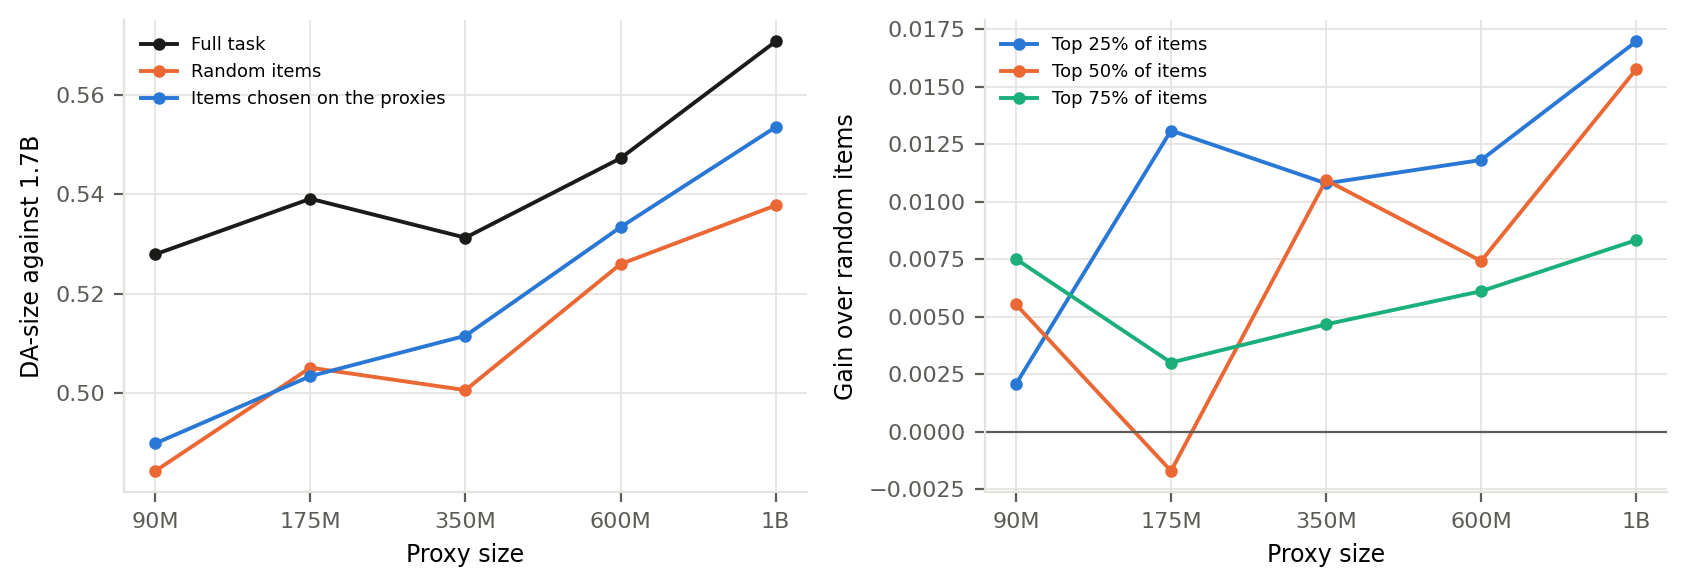
\includegraphics[width=\textwidth,height=0.36\textheight,keepaspectratio]{figures/app_rq14_proxy_item_selection.png}
% source: src/signal-and-noise/analysis/rq14_proxy_item_selection/pretraining/predictivity/proxy_item_selection_da_size_multi_axes_paper.png
\captionof{figure}{\textbf{Keeping the top half of the candidates helps little over random items.} Left: DA-size of the proxies against the 1.7B ranking on the full task, on multi-axis design pairs, for the full task (black), for random items of the same count (orange) and for the top half of the items chosen on the proxies (blue). Right: the gain of the chosen items over the random ones, one line per share of the items kept.}
\label{fig:app_rq14_proxy_item_selection}
\end{minipage}
\vspace{\baselineskip}
}]
